\documentclass[]{article}
\usepackage[utf8]{inputenc}
\usepackage{graphicx}
\usepackage{hyperref}
\usepackage{xcolor}
\usepackage{multirow}
\usepackage{float}

\title{\textbf{Stock Price and Direction Prediction via Deep Attention-Based Convolutional Neural Networks}}
\author{Onur Alaçam, Tuğcan Hoşer, Uygar Kaya, Tuna Tuncer}
\date{\textbf{2022 Spring}}

\begin{document}

\begin{figure}[h]
    \begin{center}
        
\includegraphics[]{assets/OzU.png}
    \end{center}
\end{figure}

\begin{center}
    OZYEGIN UNIVERSITY\\*
    FACULTY OF ENGINEERING\\*
    DEPARTMENT OF COMPUTER SCIENCE
\end{center}

\begin{center}
    \textbf{CS 402}\\* \vspace{0.2cm}
    \textbf{2022 Spring}\\* \vspace{0.4cm}
    \textbf{SENIOR PROJECT REPORT}\\* \vspace{0.6cm}
    \textbf{Stock Price and Direction Prediction via Deep Attention-Based Convolutional Neural Networks}\\* \vspace{0.8cm}
    \textbf{By}\\*
    \textbf{Onur Alaçam, Tuğcan Hoşer, Uygar Kaya, Tuna Tuncer}\\* \vspace{0.6cm}
    \textbf{Supervised By}\\*
    \textbf{Assistant Prof. Emre Sefer}\\* \vspace{0.6cm}
\end{center}
\textbf{Declaration of Own Work Statement/ (Plagiarism Statement)}\\*
Hereby I confirm that all this work is original and my own. I have clearly referenced/listed all sources as appropriate and given the sources of all pictures, data etc. that are not my own. I have not made any use of the essay(s) or other work of any other student(s) either past or present, at this or any other educational institution. I also declare that this project has not previously been submitted for assessment in any other course, degree or qualification at this or any other educational institution.\vspace{0.2cm}\\*
\textbf{Student Name and Surname:}\\* Onur Alaçam, Tuğcan Hoşer, Uygar Kaya, Tuna Tuncer \vspace{0.1cm}\\*
\textbf{Signature:} \vspace{0.9cm}\\*
\textbf{Place, Date:}\\* Istanbul, Turkey - 01.06.2022

\tableofcontents

\maketitle
\begin{center}
    \textbf{\Large Abstract}
\end{center}
Since stock prices are time series data, most academic studies have focused on time series forecasting in machine learning models. Unfortunately, these models do not perform as well as excepted. In this project, we converted the 1-D time-series data to 2-D images with the help of the technical indicators. Then, using these images, we compared a few state-of-the-art models in the field of computer vision such as ConvMixer, Vision Transformer, and the CNN-TA model, which is also used for predicting stock prices in the literature before. We investigated the effects of self-attention and patch embedding in the finance area. Implementations of all models are done in Tensorflow - Keras framework in the Python Programming Language.


\begin{center}
    \section{Introduction}
\end{center}
In the last decade, Machine Learning architectures have started to become popular in finance as in other fields, however, most of these architectures do not give the expected performance in the time series data with current technologies. Thus, Deep Learning architectures have recently attracted more attention. Specifically, in recent years, with the discovery of the attention mechanism, there have been crucial developments in the field of Computer Vision, hence we decided to apply this potential to the field of finance. In order to take advantage of Computer Vision models, we had to convert the time series data into images. \vspace{0.0005cm} \\*
In our research, we use the Vision Transformer architecture, which uses patch embedding and applies the attention mechanism to transformer models, and the ConvMixer architecture, which integrates the patch embeddings structure into Convolutional Neural Networks. Also, in our project, we have implemented the main architecture of the article "Algorithmic Financial Trading with Deep \textbf{Convolutional Neural Networks}"[2], in order to compare the results we will get from these architectures. \vspace{0.2cm} \\*
It's a fact for many years that the convolutional neural networks has dominated the computer vision field, but the Vision Transformer claims to outperform CNNs in most cases. It is believed that patch embedding, and self-attention mechanisms, and the complex transformer structure are crucial parts of the success of Vision Transformer. On the other hand, ConvMixer, which was released in January 2022, is claiming to perform better than both Vision Transformer and other CNN models. Moreover, the authors of the ConvMixer, claim that the success of the Vision Transformer is the result of the patch embedding mechanism rather than the complex transformer architecture of the model. Our aim is to show the effects of both patch embedding and self-attention mechanisms on the finance field by comparing these architectures. \vspace{0.2cm} \\*
As we mentioned above, we used technical indicators to obtain images from time series data for the project, each row of our images represents a different day, while each column represents a different technical indicator value. Since we used 67 different technical indicators in total, the size of our images became 67x67. By putting these images into the 3 different architectures, ConvMixer, Convolutional Neural Network, and Vision Transformer, we compared each of our models in terms of Computational Model Performance and Financial Evaluation. \vspace{0.2cm} \\*
The background will be covered in the second chapter, where we will discuss the approaches, tools, and technology that we have used in our senior project. The third chapter will discuss our problem statement and the problem we are attempting to solve. The fourth chapter will describe how we tackled the problem and how we came up with answers. In the fifth chapter, we will be examining our findings and what we were able to accomplish, and what we were unable to accomplish. We've mentioned flaws we found when looking at the outcomes in the findings, as well as how we might fix them in the future. We compare our technique and model to other comparable works in the sixth chapter. The seventh chapter contains our conclusion as well as our recommendations.

\begin{center}
    \item\section{Background}
\end{center}
The tools, technologies and various techniques used in our project are explained in detail below.\vspace{0.25cm}

\subsection{Technologies}
\textbf{Nvidia CUDA:} Nvidia Cuda is a set of development tools that enable algorithms to run on the GPU. We used Nvidia Cuda with Keras to train our models faster on GPU rather than CPU.\vspace{0.1cm}\\*
\textbf{Pandas:} Pandas is a software library written in the Python programming language for data manipulation and analysis. We processed numerical data and tables with using this library.\vspace{0.1cm}\\*
\textbf{Numpy:} NumPy is a library for the Python programming language that supports large, multidimensional arrays and matrices, adding high-level mathematical functions to operate on these arrays.\vspace{0.1cm}\\*
\textbf{TA-Lib:} TA-Lib is a library that contains 150 different indicators, especially used for trading algorithms. We also used 11 different indicators thanks to this library.\vspace{0.1cm}\\*
\textbf{TensorFlow:} TensorFlow is a free \& open source software library for machine learning. The architectures in the articles we compared used TensorFlow because they were implemented in TensorFlow.\vspace{0.1cm}\\*
\textbf{Keras:} Keras is an open source neural network library written in Python. Our architectures are implemented using Keras.\vspace{0.1cm}\\*
\textbf{Sklearn:} Scikit-learn is a free software machine learning library for the Python programming language. It is used to separate data, scale, and measure metrics as a result of the architecture.\vspace{0.1cm}\\*
\textbf{Matplotlib:} Matplotlib is a plotting library for the Python programming language and numerical math extension NumPy. We used it to visualize the results from our data.
\subsection{Indicators}
We got the data of S\&P 500 from Yahoo Finance from 2001 to 2021. We have turned these data into pictures by adhering to 11 economic technical indicators. In this part, we will talk about the indicators we have used.\vspace{0.3cm}\\*
\textbf{RSI: Relative Strength Index}\\*
The Relative Strength Index (RSI) is an indicator that provides predictions about the direction of the short and medium-term trend calculated by comparing the closing values of the relevant period with the previous closing values of the period.
\begin{figure}[H]
\begin{center}
   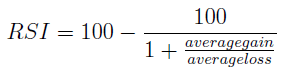
\includegraphics[width=55mm,scale=0.5]{assets/formulas/rsi.png}
   \caption{RSI Formula}
\end{center}
\end{figure}
\noindent
\textbf{WMA: Weighted Moving Average} \\*
A Weighted Moving Average puts more weight on recent data and less on past data. This is done by multiplying each bar’s price by a weighting factor. Because of its unique calculation, WMA will follow prices more closely than a corresponding Simple Moving Average.
\begin{figure}[H]
\begin{center}
   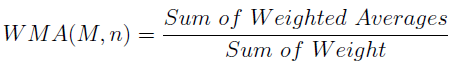
\includegraphics[width=85mm,scale=0.8]{assets/formulas/wma.png}
   \caption{WSI Formula}
\end{center}
\end{figure}
\noindent
\textbf{EMA: Exponential Moving Average} \\*
EMA, which stands for Exponential Moving Average, is used as an indicator of moving averages. Through the EMA, traders can watch exponential moving averages on the charts. By giving weight to last minute data such as EMA closing prices, the time that can progress with the weights assigned to the relevant data is based on the exponentially decreasing process.
\begin{figure}[H]
\begin{center}
   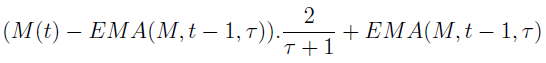
\includegraphics[width=95mm,scale=0.8]{assets/formulas/ema.png}
   \caption{EMA Formula}
\end{center}
\end{figure}
\noindent
\textbf{SMA: Simple Moving Average} \\*
Simple Moving Average (SMA) is the simplest form of moving averages. It is obtained by dividing the total of data by the number of data.
\begin{figure}[H]
\begin{center}
   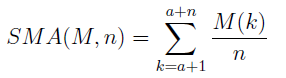
\includegraphics[width=55mm,scale=0.8]{assets/formulas/sma.png}
   \caption{SMA Formula}
\end{center}
\end{figure}
\noindent
\textbf{ROC: Rate of Change}\\*
The Rate of Change Indicator (ROC) is a kind of momentum oscillator. Calculates the rate of price change between periods.
\begin{figure}[H]
\begin{center}
   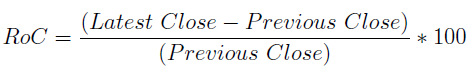
\includegraphics[width=80mm,scale=0.8]{assets/formulas/roc.png}
   \caption{ROC Formula}
\end{center}
\end{figure}
\noindent
\textbf{CMO: Chande Momentum Oscilator Indicator} \\*
The Chande Momentum Oscillator (CMO) is calculated by dividing the sum of the momentum on the up days and the sum of the momentum on the down days by dividing the sum of the momentum on the up days by the sum of the momentum on the down days and multiplying by 100 to make a percentage.
\begin{figure}[H]
\begin{center}
   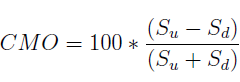
\includegraphics[width=45mm,scale=0.8]{assets/formulas/cmo.png}\\*
   \textit{$S_U$: Total momentum of the up days for the analysis period}\vspace{0.1cm}\\*
   \textit{$S_D$: Total momentum of the down days for the analysis period}\vspace{0.2cm}\\*
   \caption{CMO Formula}
\end{center}
\end{figure}
\noindent
\textbf{CCI: Commodity Channel Index} \\*
Commodity Channel Index (CCI) is an indicator that compares current prices and the average price over a period of time.
\begin{figure}[H]
\begin{center}
   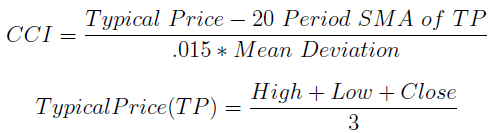
\includegraphics[width=80mm,scale=0.8]{assets/formulas/cci.png}
   \caption{CCI Formula}
\end{center}
\end{figure}
\noindent
\textbf{PPO: Percentage Price Oscillator} \\*
The Percentage Price Oscillator (PPO) is a technical momentum indicator that displays the relationship between two moving averages in percentage terms. The moving averages are the 26-period and 12-period exponential moving average (EMA).
\begin{figure}[H]
\begin{center}
   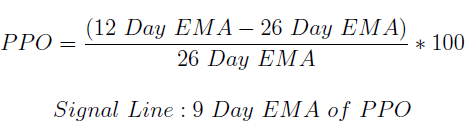
\includegraphics[width=80mm,scale=0.8]{assets/formulas/ppo.png}
   \caption{PPO Formula}
\end{center}
\end{figure}
\noindent
\textbf{TEMA: Triple Exponential Moving Average} \\*
Triple Exponential Moving Average (TEMA) is a type of EMA indicator that provides the reduction of minor price fluctuations and filters out volatility.
\begin{figure}[H]
\begin{center}
   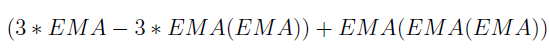
\includegraphics[width=90mm,scale=0.8]{assets/formulas/tema.png}
   \caption{TEMA Formula}
\end{center}
\end{figure}
\noindent
\textbf{WILLR: Williams} \\*
Williams \%R, also known as the Williams Percent Range, is a type of momentum indicator that moves between 0 and -100 and measures overbought and oversold levels.
\begin{figure}[H]
\begin{center}
    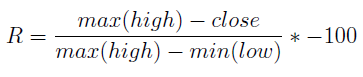
\includegraphics[width=75mm,scale=0.8]{assets/formulas/willr.png}
    \caption{WILLR Formula}
\end{center}
\end{figure}
\noindent
\textbf{MACD: Moving Average Convergence and Divergence} \\*
The Moving Average Convergence and Divergence (MACD) indicator is a technical indicator that displays how stock values are trending.
\begin{figure}[H]
\begin{center}
    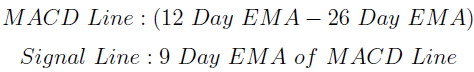
\includegraphics[width=80mm,scale=0.8]{assets/formulas/macd.png}
    \caption{MACD Formula}
\end{center}
\end{figure}
\subsection{ETFs}
\textbf{Yahoo Finance:} Yahoo Finance provides financial news, data and commentary including stock quotes, press releases, financial reports, and original content. We downloaded the S\&P 500 dataset from here. In addition, we will consider companies individually in the future and we plan to download their data from Yahoo Finance.\vspace{0.1cm}\\*
\textbf{S\&P:} The S\&P 500 includes major American companies. It covers about 75\% of the American stock market. We used data from the last 21 years of S\&P.\vspace{0.1cm}\\*
\textbf{XLF:} The Financial Select Sector SPDR Fund (XLF) is a diversified fund with many blue-chip companies in its portfolio. It covers a variety of industries within the financial sector, has generated strong returns, has high liquidity, and is a medium-cost investment. \vspace{0.1cm}\\*
\textbf{XLU:} The Utilities Select Sector SPDR® Fund seeks to provide investment results that, before expenses, correspond generally to the price and yield performance of the Utilities Select Sector Index. \newline Seeks to provide precise exposure to companies from the electric utility, water utility, multi-utility, independent power and renewable electricity producers, and gas utility industries. \vspace{0.1cm}\\*
\textbf{QQQ:} The Invesco QQQ ETF is an exchange-traded fund (ETF) that tracks the Nasdaq 100 Index. Because it passively follows the index, the QQQ share price goes up and down along with the tech-heavy Nasdaq 100 \vspace{0.1cm}\\*
\textbf{XLP:} The Consumer Essentials Industry SPDR\® Fund aims to provide investment results that correspond to the price and yield performance of the Consumer Essentials Industry Index, prior to expenditure. The Index aims to provide an effective representation of the S&P 500 Index's core consumer products sector.\vspace{0.1cm}\\*
\textbf{EWZ:} EWZ tracks the MSCI Brazil 25/50 Index, which provides a broad-based measure of the performance of the Brazilian equity market.7 The ETF provides exposure to midcap and large-cap companies based in Brazil. Its largest allocations are in the materials, financial, energy sectors of the Brazilian economy. \vspace{0.1cm}\\*
\textbf{EWH:} Shares, Inc. - iShares MSCI Hong Kong ETF is an exchange traded fund launched by BlackRock, Inc. It is managed by BlackRock Fund Advisors. It invests in public equity markets of Hong Kong. The fund invests in stocks of companies operating across diversified sectors. It invests in growth and value stocks of companies across diversified market capitalization. \vspace{0.1cm}\\*
\textbf{XLY:} The Consumer Discretionary Select Sector SPDR® Fund seeks to provide investment results that, before expenses, correspond generally to the price and yield performance of the Consumer Discretionary Select Sector Index. Seeks to provide precise exposure to companies in retail (specialty, multiline, internet and direct marketing); hotels, restaurants and leisure; textiles, apparel and luxury goods; household durables; automobiles; auto components; distributors; leisure products; and diversified consumer services. \vspace{0.1cm}\\*
\textbf{XLE:} One of the most popular exchange-traded funds (ETFs) used by retail traders seeking exposure to energy is the Energy Select Sector SPDR Fund, which tracks the S\&P Energy Select Sector Index.
\noindent
\begin{center}
    \item\section{Problem Statement}
\end{center}
\subsection{Project Scope}
Our problem was that today's machine learning models were inadequately effective in the area of finance since the majority of today's models struggled with time-series data because time introduces a new piece of information that must be monitored. In addition, many successful studies have been carried out in the world of deep learning in recent years, and these studies have led to successful results in the literature. Our goal was to see if advanced deep learning techniques like patch embedding and self-attention, which have just recently been introduced, can achieve the anticipated results when applied to finance.
The majority of the strategies we employ in our project may be found in the article Algorithmic Financial Trading. In addition to this research, we included the following in our project: While the AFT paper produced findings using a single form of CNN, we acquired results with two additional freshly designed alternative architectures and compared them to the results in the article. Also, we explored how various topologies of these architectures would operate in our problem. Moreover, while the AFT article employed 15 technical indicators, we added 67 technical indications to increase the size of our picture.

\subsection{Engineering Problem}
Although finance problems often deal with time-series data, we have transformed our problem into an image classification problem rather than a time-series forecasting problem by turning time-series data into images. One of the issues we encountered was the proper evaluation of our models. Because our dataset was distributed in an imbalanced manner in one of the configurations we employed, we had to seek several metrics in order to appropriately evaluate the success of our model. Furthermore, when we couldn't obtain the results we wanted with 11x11 images, we decided to increase the number of technical indicators and make our images 67x67 because the attention mechanism used in the vision transformer worked on the logic of focusing on the key elements of the large image. As a result, we sought to make our image as large as possible.

\subsection{Assumptions and Constraints}
Since only technical indicators are used in the data creation process in this project, we assume that stock prices can only be modeled with technical indicators. However, as is well known, today's stock values are heavily influenced by a variety of events such as wars, legislation, and tweets. As a result, cryptocurrency volatility is substantially higher than stock market index volatility. This is why we decided to focus our analysis on stocks rather than cryptocurrency. \vspace{0.1cm} \newline
We chose to conduct this project with our supervisor, Assistant Prof. Emre Sefer. Following that, we carried out extensive research into the problem and discussed potential improvements. \vspace{0.1cm} \newline
We calculated the correlation of all technical indicators according to RSI when constructing the images since the order in which they are arranged would impact the model's learning. Following that, we arranged the indicators in this correlation order.
\begin{center}
    \item\section{Solution Approach}
\end{center}
\subsection{Dataset Preparation}
First and foremost, we had to decide whether we would proceed with our work on stocks or cryptocurrencies.\vspace{0.2cm}\\*
Due to the high volatility of cryptocurrencies, the accuracy of the predictions to be made with the models could be lower. Because, in today's cryptocurrency market, which can change rapidly with the tweets of celebrities, our work could be more challenging. That's why we decided to make predictions on stocks.\vspace{0.01cm} \\*
In the paper \textit{Algorithmic Financial Trading with Deep Convolutional Neural Networks: Time Series to Image Conversion Approach} [2], it was reported that models with ETF data outperformed the models with Dow30 data in terms of accuracy. That's why we decided to use ETFs from this paper. We also wanted to include the 2008 economic crisis so that our dataset does not exhibit an entirely increasing market trend. As a result, we generated our dataset utilizing data from 2001-10-11 to 2022-04-15.\vspace{0.1cm}\\*
After we created our dataset, we converted it into images to use in our architectures. We constructed our images by using 11 of the 15 indicators described in the paper \textit{Algorithmic Financial Trading with Deep Convolutional Neural Networks: Time Series to Image Conversion Approach} [2]. Apart from the article, we used 56 more indicators and our total number of indicators became 67. As a result, our photos are 67x67 in size.
We also arranged the order in which the indicators will be placed on the image by looking at the correlation values between the indicators. Because different ordering will lead to different images this might have affected the performance of models.
Each image was created using 67 days of historical data from 67 indicators. As an example, if we are on day t and wish to anticipate what will happen on day t+1, the image will be constructed utilizing indicators from day t through day t-66.\vspace{0.1cm}\\*
Furthermore, we had to decide on a threshold value for labeling the dataset. Figure 19 depicts the algorithm for labeling photos using the threshold. In short, we decided to label an image as buy if the price increased more than the set threshold, sell if the price dropped more than the threshold, and hold if not both.
In the labeling process of our images, also as presented in Table 1, we decided to construct two separate label sets utilizing two different thresholds. We selected 0.0038 as the threshold value since we wanted to spread the data as evenly as possible. Thus we were able to generate predictions based on a balanced dataset. On the other hand, we picked 0.01 as our threshold with financial reasons in mind since we concluded that if the stock's value increases by 1\% in a day, it's a good idea to purchase it ahead of time, and if it decreases by 1\%, it's a good idea to sell it beforehand. Furthermore, a value of 0.0038 lays the foundation for a higher-frequency trading strategy, whereas the value of 0.01 generates more hold-centric predictions and is akin to a buy\&hold strategy. Finally, to improve the accuracy of the models we will train, we scaled our data such that the standard deviation is one and the mean is zero.\vspace{0.1cm}\\*
\begin{table}[H]
\centering
    \caption{Label Distribution by Different Threshold Values}
\begin{tabular}{|l|c|c|c|l|l|l|}
\hline
Threshold & \multicolumn{1}{l|}{Buy} & \multicolumn{1}{l|}{Hold} & \multicolumn{1}{l|}{Sell} & Buy \% & Hold \% & Sell \% \\ \hline
0.0038     & 13174                     & 11461                      & 11437                      & 36.5\% & 31.8\%  & 31.7\%  \\ \hline
0.01      & \multicolumn{1}{l|}{6547} & \multicolumn{1}{l|}{23486} & \multicolumn{1}{l|}{6039}  & 18.1\% & 65.1\%  & 16.8\%  \\ \hline
\end{tabular}
\end{table}
\subsection{Implementing Different Architectures \& Training the Models}
The results from part 1 of how our data is retrieved, processed, and transformed heavily influences this section. A total of three different architectures were used in this project. These architectures are Convolutional Neural Networks (CNN-TA), ConvMixer and Vision Transformer, respectively. By training the data from Part 1 on these three different architectures, the results obtained for each architecture were compared.\vspace{0.1cm} \\*
In this senior peoject, different hyperparameters are selected for each different architecture.\vspace{0.3cm} \\*
\textbf{\large Convolutional Neural Networks} \\*
In our proposed CNN analysis phase, as can be seen in Figure, nine layers are used. These are listed as follows: input layer (67x67), two convolutional layers (67x67x32, 67x67x64), a max pooling (33x33x64), two dropout (0.25, 0.50), fully connected layers (128), and an output layer (3).
\begin{figure}[H]
\begin{center}
   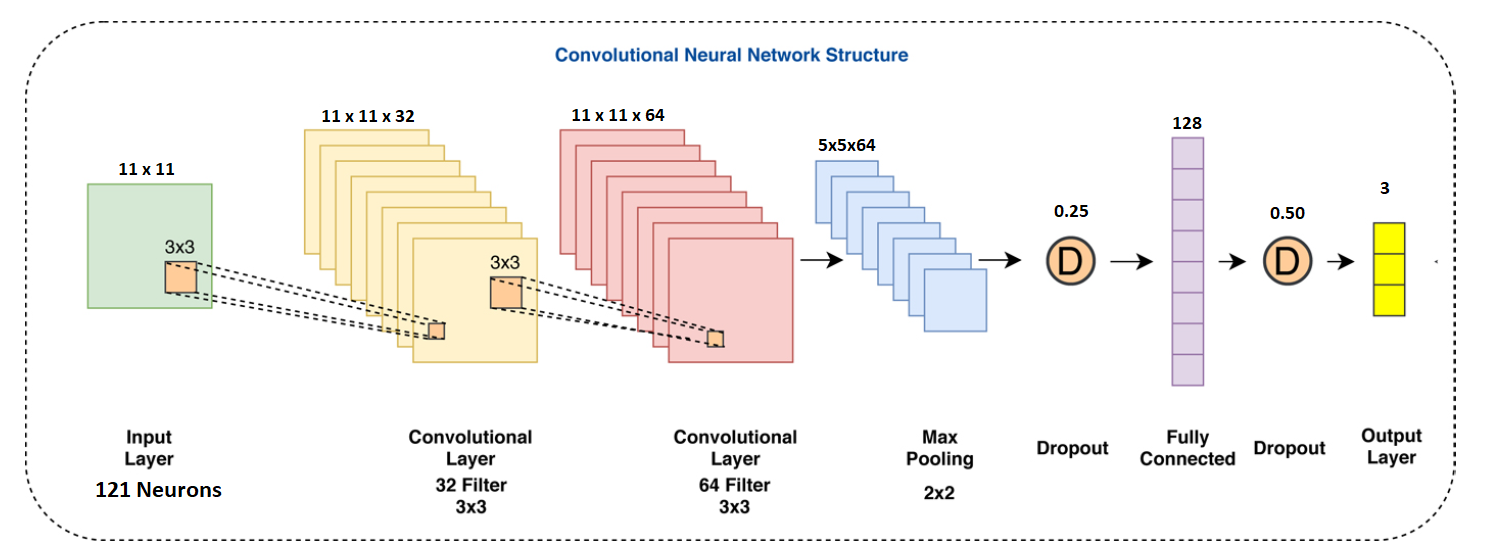
\includegraphics[scale=0.24]{assets/structures/cnn.png}
   \caption{Convolutional Neural Network Structure}
\end{center}
\end{figure}
\noindent
By using an image filter in the convolution layer, we enlarge the channel of the image with stride and padding operations. The filter is generally chosen as 3x3, 5x5 or 7x7. We opted not to adjust the kernel size since Sezer and Ozbayoglu (2018) used a kernel size of 5x5 in their models. In this way, when we apply 2 convolution layers on the 67x67 image, we get an 67x67x64 image. Then we pass it through the max pooling layer, and we get a 33x33x64 image. \newline Dropout layers are added to prevent overfitting. By reducing the final image to one dimension, we get 128 fully connected neural networks. Then we transform these neural networks into our class labels \textbf{Buy}, \textbf{Hold} \& \textbf{Sell} outputs on the output layer.\vspace{0.1cm} \\*
We used Keras while implementing CNN. Although we have two different labelsets, we kept all our hyperparameter values same during the training of the model for two different threshold values. We also utilized Ada Delta, which was developed by Zeiler Matthew (2012) and was used in the Algorithmic Financial Trading paper, as the optimizer.\vspace{0.3cm} \\*
\textbf{\large ConvMixer}
\begin{figure}[H]
\begin{center}
    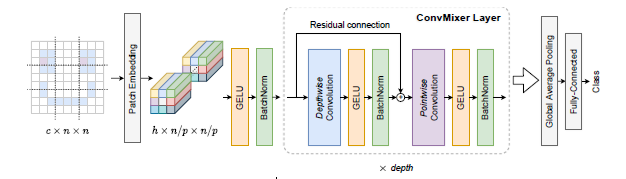
\includegraphics[scale=0.7]{assets/structures/convmixer.png}
    \caption{ConvMixer Structure}
\end{center}
\end{figure}
\noindent
In ConvMixer, we first split the image into patches by applying patch embedding. Then, we pass each patch through the GELU [\textit{Equation 1}] and Batch Normalization [\textit{Equation 2}] layers separately as an activation function. We pass the resulting patches through the ConvMixer layer. The ConvMixer layer contains Depthwise Convolution, activation function, Pointwise Convolution and activation function, respectively. Depthwise Convolution is a sort of convolution in which each input channel receives a single convolutional filter and Pointwise Convolution is a form of convolution that uses a 1x1 kernel, which iterates through each point.\vspace{0.2cm}\\*
We used tensorflow and keras while implementing ConvMixer. In order to select the hyperparameters optimally, we trained the images by giving different numbers of epoch, batch size, patch size, kernel size and learning rate. As a result, we trained a 256x8 model for 166 epochs using kernel size, patch size of 5, and batch size of 128 on our dataset with a threshold value of 0.0038. Moreover, we trained a 128x8 model for 114 epochs using a kernel size of 7, patch size of 2, and batch size of 32 on our dataset with a threshold value of 0.01. Also for both configurations, we utilized Ada Delta as the optimizer.\vspace{0.2cm} \\*
\textit{Equation 1:} $GELU(x)=xP(X \leq x)=x \phi (x)$ \vspace{0.1cm}\\*
\textit{Equation 2:} $y = ((x - E[x])/\sqrt{Var[x]+\epsilon}) \hspace{0.1cm} \DeclareMathSymbol{*} \hspace{0.1cm} \gamma + \beta$ \vspace{0.7cm} \\*
\textbf{\large Vision Transformer} \\*
\begin{figure}[H]
\begin{center}
    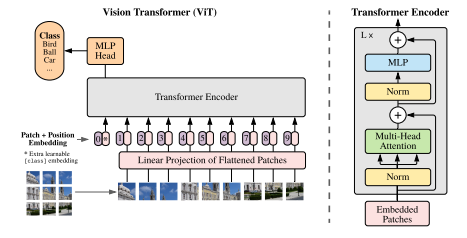
\includegraphics[scale=0.4]{assets/structures/visionTransformer.png}
    \caption{Vision Transformer Structure}
\end{center}
\end{figure}
\noindent
In the Visual Transformer model, the normal transformer model is adapted to the images. 2D images are converted into sequence of flattened 2D patches using patch + position embedding. Then these patches are given to the transformer encoder according to their positions. Transformer Encoder contains 3 layers, these layers are Normalization, Multi-Head Attention, Normalization. Multi-Head Attention is an attention mechanism module that runs through an attention mechanism multiple times in parallel. After the patches pass through these layers, a classification model, MLP, has been added for the classification to take place. We used tensorflow and keras while implementing Vision Transformer. Finally, we preferred the same hyperparameters for both threshold values. We got patch size as 11, transformer layer as 10, number of heads as 4, and projection dimension as 64. We employed one cycle scheduler as a learning rate scheduler while utilizing AdamW as an optimizer. The weight decay was 0.0001 and the base learning rate was 0.002.
\subsection{Technical, Operational \& Financial Feasibility}
\textbf{Technical Feasibility} \vspace{0.1cm}\\*
In general, Deep Learning architectures take excessively extended to train, therefore we trained our models on the GPU instead of the CPU in our senior project. When we are going to use the CPU, we have trained the models that we can train for days or weeks, in theory, using NVIDIA CUDA for an average of 8-10 hours.\vspace{0.2cm}\\*
\textbf{Financial Feasibility} \vspace{0.1cm}\\*
We don't have any other cost without needing a better performing and equipped computer to train our model.
\subsection{Knowledge \& Skill Set}
Different skill sets from various courses were used in our senior project. While the courses mentioned here had the most impact on our project, all the CS courses we've reviewed so far have given us new perspectives in implementing this project.\vspace{0.2cm} \\*
\textbf{CS 101:} The basics of programming were learned and helped to use the basic knowledge in this project.\vspace{0.1cm} \\*
\textbf{CS 320:} Helped us to design and write the project reports accurately.\vspace{0.1cm}\\*
\textbf{CS 447:} Helped us to request Yahoo Finance data. \vspace{0.1cm}\\*
\textbf{CS 452:} Helped us to create and pre-process the dataset as well as apply the classification model. \vspace{0.1cm}\\*
\textbf{CS 454:} Helped us to understand the neural network logic and its pros and cons. \vspace{0.1cm}\\*
\textbf{MATH 211:} Helped us to understand the matrices in the structure of the images. \vspace{0.1cm} \\*
\textbf{MATH 217:} Help us to compare statistics in results.
\subsection{Engineering Standards}
• Style Guide for Python Code\\*
• Data Format: NumPy Array\\*
• HTTP Protocols: GET

\begin{center}
    \item\section{Results and Discussion}
\end{center}
We attempted to obtain results with the ConvMixer, Vision Transformer and CNN-TA architectures using the dataset we generated. Since our dataset is different from the Algorithmic Financial Trading paper, the results we got were also different. We decided to use two different strategies, computational model performance evaluation and financial evaluation, to evaluate performance. In the performance section of the computational model, metrics such as accuracy, recall, precision, and f1 score are used to assess neural network performance; in the financial evaluation section, metrics such as return and sharpe ratio are used to assess the model's financial success. As previously stated, since we trained the models using two separate threshold values, the results for both the 0.01 and 0.0038 threshold values are presented in detail below. \vspace{0.2cm} \\*
As we observed an increase in validation loss in ConvMixer and Vision Transformer architectures while training the models, we noticed that these models were overfitted. That's why we trained the ConvMixer at 200 epochs and the Vision Transformer at 100 epochs. Since we did not encounter such a problem in the CNN architecture, we trained the model at 500 epochs. \vspace{0.2cm}\\*

%{To begin with, one of the most significant findings was that the distribution of predictions in the ConvMixer architecture was more diversified than that of the Vision Transformer architecture. The ConvMixer model assessed the buy points more accurately than the Vision Transformer model, as demonstrated by the confusion matrices in Table 1 and Table 3. While the Vision Transformer model performed better in hold predictions, both models accurately identified 18 pictures in sell. Because 49.8 percent of our dataset is labeled hold, a model is more likely to predict hold correctly. Therefore, the fact that the ConvMixer model has a better prediction percentage than the Vision Transformer for buy labeled images may indicate that the ConvMixer model is more resistant to imbalanced datasets.}

\subsection{Computational Model Performance}
\subsubsection{Threshold Value - 0.01}
\begin{figure}[H]
    \begin{center}
        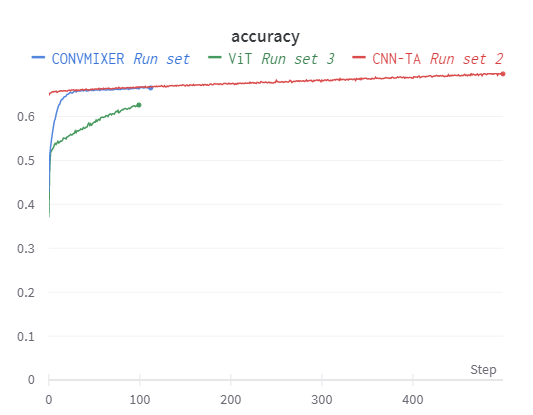
\includegraphics[scale=0.9]{assets/graphs/01/01acc.png}
        \caption{Train Accuracy Graph}
    \end{center}
\end{figure}
When we look at the Figure 15, we can see that CNN-TA started with a high accuracy value, while ConvMixer and Vision Transformer started with a lower accuracy value, but in the following epochs, ConvMixer and CNN-TA reached a very similar Train Accuracy value. However, it is less accurate than ViT, ConvMixer, and CNN-TA.
\begin{figure}[H]
    \begin{center}
        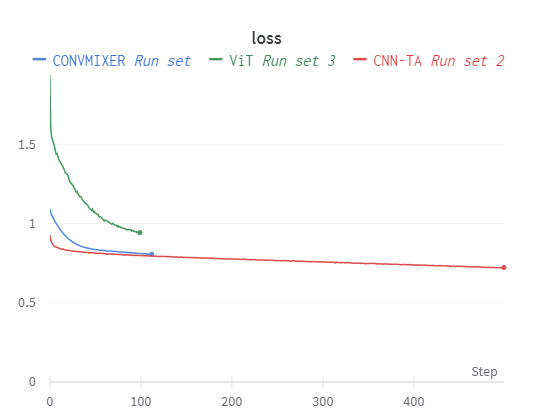
\includegraphics[scale=0.9]{assets/graphs/01/01loss.png}
        \caption{Train Loss Graph}
    \end{center}
\end{figure}
\noindent
As seen in the Figure 16, when we look at the Loss values in the graphics where we took the Threshold value as 0.01, in the first epochs, CNN-TA starts from the low loss value, ConvMixer starts from a higher loss value than CNN-TA, also Vision Transformer starts at a higher value than ConvMixer. In following epochs, ConvMixer has achieved a very similar loss with CNN-TA, but ViT remains higher than ConvMixer and CNN-TA. \vspace{0.1cm}
\begin{figure}[H]
    \begin{center}
        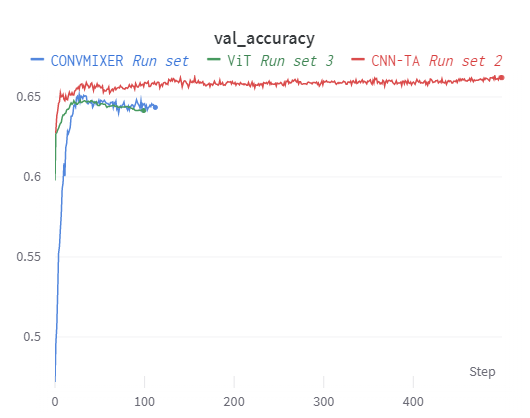
\includegraphics[scale=0.9]{assets/graphs/01/01valacc.png}
        \caption{Validation Accuracy Graph}
    \end{center}
\end{figure}
\noindent
In Figure 17, when we compare the validation accuracy rates of three different architectures, we see that ConvMixer and CNN-TA have oscillation, but as seen in the graph, we see that the highest validation accuracy is in CNN-TA.
\begin{figure}[H]
    \begin{center}
        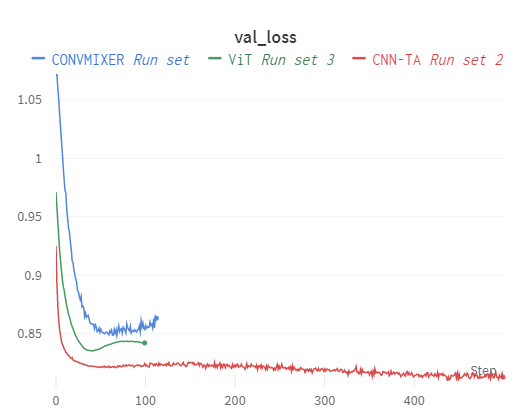
\includegraphics[scale=0.9]{assets/graphs/01/01valloss.png}
        \caption{Validation Loss Graph}
    \end{center}
\end{figure}
\noindent
In the Figure 18, when we look at the validation loss values in the graphics where we took the Threshold value as validation loss value, ConvMixer starts from a highest validation loss value. Also Vision Transformer starts at a higher value than CNN-TA.There is an increase in validation loss values in ConvMixer and ViT around the 50th epoch and it is seen that they are slightly overfitting. In addition, oscillations are clearly evident in ConvMixer and CNN-TA. \vspace{0.2cm} \\* 
\textbf{ConvMixer:}
\begin{table}[H]
    \centering
    \caption{Confusion Matrix of ConvMixer}
    \begin{tabular}{llcccll}
        \cline{1-5}
        \multicolumn{1}{|l|}{} & \multicolumn{1}{l|}{} & \multicolumn{3}{c|}{Predicted} & & \\\cline{1-5} \multicolumn{1}{|l|}{} & \multicolumn{1}{l|}{} & \multicolumn{1}{l|}{Buy} & \multicolumn{1}{l|}{Hold} & \multicolumn{1}{l|}{Sell} & & \\ \cline{1-5} \multicolumn{1}{|c|}{\multirow{3}{*}{Actual}} & \multicolumn{1}{l|}{Buy} & \multicolumn{1}{c|}{130} & \multicolumn{1}{c|}{1620} & \multicolumn{1}{c|}{47} & & \\ \cline{2-5} \multicolumn{1}{|c|}{} & \multicolumn{1}{l|}{Hold} & \multicolumn{1}{c|}{64} & \multicolumn{1}{c|}{5513}  & \multicolumn{1}{c|}{48}& & \\ \cline{2-5} \multicolumn{1}{|c|}{} & \multicolumn{1}{l|}{Sell} & \multicolumn{1}{c|}{107} & \multicolumn{1}{c|}{1452} & \multicolumn{1}{c|}{37} & & \\ \cline{1-5} & & \multicolumn{1}{l}{} & \multicolumn{1}{l}{} & \multicolumn{1}{l}{} &&
    \end{tabular}
\end{table}

\begin{table}[H]
\centering
\caption{Classification Report of ConvMixer}
\begin{tabular}{|llll|}
\hline
\multicolumn{4}{|c|}{\textbf{Test Accuracy: 0.6299}}                                                         \\ \hline
\multicolumn{1}{|l|}{}               & \multicolumn{1}{l|}{Buy}  & \multicolumn{1}{l|}{Hold} & Sell \\ \hline
\multicolumn{1}{|l|}{Recall}         & \multicolumn{1}{l|}{0.07} & \multicolumn{1}{l|}{0.98} & 0.02 \\ \hline
\multicolumn{1}{|l|}{Precision}      & \multicolumn{1}{l|}{0.43} & \multicolumn{1}{l|}{0.64} & 0.28 \\ \hline
\multicolumn{1}{|l|}{F1 Score}       & \multicolumn{1}{l|}{0.12} & \multicolumn{1}{l|}{0.78} & 0.04 \\ \hline
\multicolumn{1}{|l|}{Weighted Prec.} & \multicolumn{3}{c|}{0.5362}                                  \\ \hline
\multicolumn{1}{|l|}{Weighted F1}    & \multicolumn{3}{c|}{0.5163}                                  \\ \hline
\end{tabular}
\end{table}

\textbf{Vision Transformer:}
\begin{table}[H]
    \centering
    \caption{Confusion Matrix of Vision Transformer}
    \begin{tabular}{llcccll}
        \cline{1-5}
        \multicolumn{1}{|l|}{} & \multicolumn{1}{l|}{} & \multicolumn{3}{c|}{Predicted} & & \\\cline{1-5} \multicolumn{1}{|l|}{} & \multicolumn{1}{l|}{} & \multicolumn{1}{l|}{Buy} & \multicolumn{1}{l|}{Hold} & \multicolumn{1}{l|}{Sell} & & \\\cline{1-5} \multicolumn{1}{|c|}{\multirow{3}{*}{Actual}} & \multicolumn{1}{l|}{Buy} & \multicolumn{1}{c|}{73} & \multicolumn{1}{c|}{1690} & \multicolumn{1}{c|}{34} & & \\\cline{2-5} \multicolumn{1}{|c|}{} & \multicolumn{1}{l|}{Hold} & \multicolumn{1}{c|}{57} & \multicolumn{1}{c|}{5528} & \multicolumn{1}{c|}{40} & & \\\cline{2-5} \multicolumn{1}{|c|}{} & \multicolumn{1}{l|}{Sell} & \multicolumn{1}{c|}{57} & \multicolumn{1}{c|}{1517} & \multicolumn{1}{c|}{22} & & \\\cline{1-5} & & \multicolumn{1}{l}{} & \multicolumn{1}{l}{} & \multicolumn{1}{l}{} & & 
    \end{tabular}
\end{table}
\begin{table}[H]
\centering
\caption{Classification Report of Vision Transformer}
\begin{tabular}{|llll|}
\hline
\multicolumn{4}{|c|}{\textbf{Test Accuracy: 0.6235}}                                                         \\ \hline
\multicolumn{1}{|l|}{}               & \multicolumn{1}{l|}{Buy}  & \multicolumn{1}{l|}{Hold} & Sell \\ \hline
\multicolumn{1}{|l|}{Recall}         & \multicolumn{1}{l|}{0.04} & \multicolumn{1}{l|}{0.98} & 0.01 \\ \hline
\multicolumn{1}{|l|}{Precision}      & \multicolumn{1}{l|}{0.39} & \multicolumn{1}{l|}{0.63} & 0.23 \\ \hline
\multicolumn{1}{|l|}{F1 Score}       & \multicolumn{1}{l|}{0.07} & \multicolumn{1}{l|}{0.77} & 0.03 \\ \hline
\multicolumn{1}{|l|}{Weighted Prec.} & \multicolumn{3}{c|}{0.5131}                                  \\ \hline
\multicolumn{1}{|l|}{Weighted F1}    & \multicolumn{3}{c|}{0.4995}                                  \\ \hline
\end{tabular}
\end{table}
\noindent
%{In Table 5, it is seen that 89.9 percent of the test datasets are labeled as hold. This demonstrates that the dataset used for CNN-TA is much more imbalanced than our dataset. In addition, while the CNN-TA model was evaluated with 33714 test data, the test data we used to evaluate our ConvMixer and Vision Transformer models consisted of 496 images. This may explain why the total accuracy of our models is lower than that of CNN-TA and why both models are subject to overfitting very quickly.\vspace{0.2cm}\\*}
\textbf{CNN-TA:}
\begin{table}[H]
    \centering
    \caption{Confusion Matrix of CNN-TA}
    \begin{tabular}{llcccll}
        \cline{1-5}
        \multicolumn{1}{|l|}{} & \multicolumn{1}{l|}{} & \multicolumn{3}{c|}{Predicted} & & \\\cline{1-5} \multicolumn{1}{|l|}{} & \multicolumn{1}{l|}{} & \multicolumn{1}{l|}{Buy} & \multicolumn{1}{l|}{Hold} & \multicolumn{1}{l|}{Sell} & & \\\cline{1-5} \multicolumn{1}{|c|}{\multirow{3}{*}{Actual}} & \multicolumn{1}{l|}{Buy} & \multicolumn{1}{c|}{82} & \multicolumn{1}{c|}{1626} & \multicolumn{1}{c|}{89} & & \\\cline{2-5} \multicolumn{1}{|c|}{} & \multicolumn{1}{l|}{Hold} & \multicolumn{1}{c|}{45} & \multicolumn{1}{c|}{5500} & \multicolumn{1}{c|}{80} & & \\\cline{2-5} \multicolumn{1}{|c|}{} & \multicolumn{1}{l|}{Sell} & \multicolumn{1}{c|}{54} & \multicolumn{1}{c|}{1450} & \multicolumn{1}{c|}{92} & & \\\cline{1-5} & & \multicolumn{1}{l}{} & \multicolumn{1}{l}{} & \multicolumn{1}{l}{} & & 
    \end{tabular}
\end{table}

\begin{table}[H]
\centering
\caption{Classification Report of CNN-TA}
\begin{tabular}{|llll|}
\hline
\multicolumn{4}{|c|}{\textbf{Test Accuracy: 0.6292}}                                                         \\ \hline
\multicolumn{1}{|l|}{}               & \multicolumn{1}{l|}{Buy}  & \multicolumn{1}{l|}{Hold} & Sell \\ \hline
\multicolumn{1}{|l|}{Recall}         & \multicolumn{1}{l|}{0.05} & \multicolumn{1}{l|}{0.98} & 0.06 \\ \hline
\multicolumn{1}{|l|}{Precision}      & \multicolumn{1}{l|}{0.45} & \multicolumn{1}{l|}{0.64} & 0.35 \\ \hline
\multicolumn{1}{|l|}{F1 Score}       & \multicolumn{1}{l|}{0.08} & \multicolumn{1}{l|}{0.77} & 0.10 \\ \hline
\multicolumn{1}{|l|}{Weighted Prec.} & \multicolumn{3}{c|}{0.5527}                                  \\ \hline
\multicolumn{1}{|l|}{Weighted F1}    & \multicolumn{3}{c|}{0.5172}                                  \\ \hline
\end{tabular}
\end{table}
\noindent
%{In addition, as mentioned above, the size of the dataset we prepared was considerably smaller than the size of the dataset prepared for the CNN-TA model. This may have caused our models to experience rapid overfitting. In order to minimize overfitting, we plan to increase the number of data points and perform cross-validation in the future. \vspace{0.2cm}\\*}
\subsubsection{Threshold Value - 0.0038}
\begin{figure}[H]
    \begin{center}
        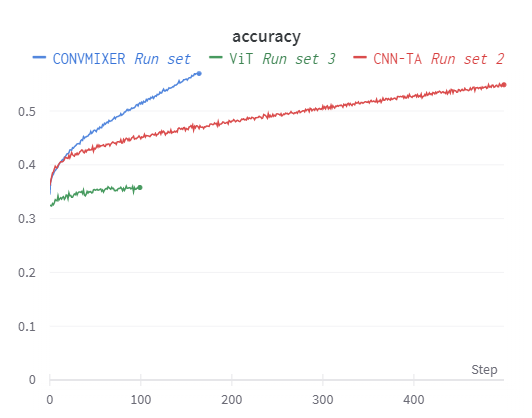
\includegraphics[scale=0.9]{assets/graphs/0038/0038acc.png}
        \caption{Train Accuracy Graph}
    \end{center}
\end{figure}
\noindent
When we look at the graphic in Figure 19, we observe that Vision Transformer starts low compared to other architectures and does not increase much. ConvMixer and CNN start with close values, but then ConvMixer rises to higher values in less epochs. CNN-TA achieves almost the same train accuracy as ConvMixer at the end of the 500 epoch.
\begin{figure}[H]
    \begin{center}
        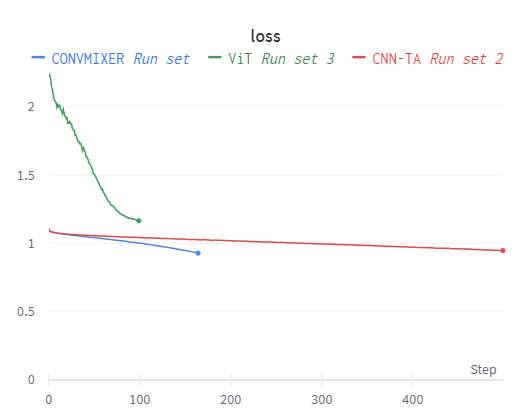
\includegraphics[scale=0.9]{assets/graphs/0038/0038loss.png}
        \caption{Train Loss Graph}
    \end{center}
\end{figure}

\noindent
As seen in the Figure 20, when we look at the loss values in the graphics where we took the threshold value as 0.0038, in the first epochs, ViT starts from the high loss value, ConvMixer starts same with CNN-TA. In following epochs, There was a decrease in loss values in all three models. However, the decrease in ViT was more sharp than the others.
\begin{figure}[H]
    \begin{center}
        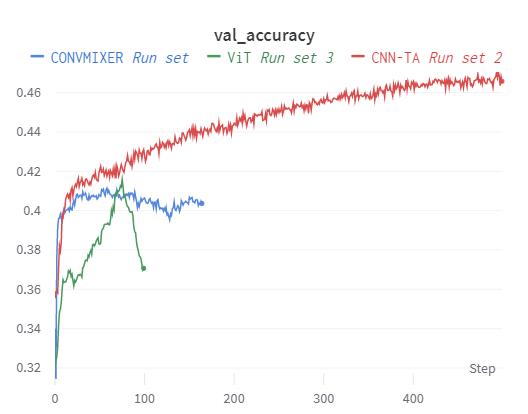
\includegraphics[scale=0.9]{assets/graphs/0038/0038valacc.png}
        \caption{Validation Accuracy Graph}
    \end{center}
\end{figure}

\noindent
As seen in Figure 21, it starts with the same validation accuracy values in all three architectures. But then, as CNN continues to rise, ConvMixer is slightly overfitted and Vision Transformer is heavily overfitted.

\begin{figure}[H]
    \begin{center}
        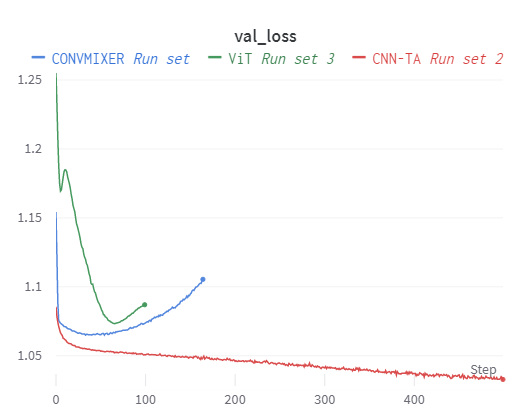
\includegraphics[scale=0.9]{assets/graphs/0038/0038valloss.png}
        \caption{Validation Loss Graph}
    \end{center}
\end{figure}

\noindent
When we look at the graphic in Figure 22, initially, the validation loss value in ViT is the highest, while ConvMixer has the second highest value and CNN has the lowest. There was a decrease in the validation loss value in all three models. ConvMixer passed ViT in validation loss value after a certain period of time. In addition, overfitting is clearly seen in these 2 models. On the other hand, CNN validation loss value decreased stably. \vspace{0.2cm}\\*
\textbf{ConvMixer:}
\begin{table}[H]
    \centering
    \caption{Confusion Matrix of ConvMixer}
    \begin{tabular}{llcccll}
        \cline{1-5}
        \multicolumn{1}{|l|}{} & \multicolumn{1}{l|}{} & \multicolumn{3}{c|}{Predicted} & & \\\cline{1-5} \multicolumn{1}{|l|}{} & \multicolumn{1}{l|}{} & \multicolumn{1}{l|}{Buy} & \multicolumn{1}{l|}{Hold} & \multicolumn{1}{l|}{Sell} & & \\ \cline{1-5} \multicolumn{1}{|c|}{\multirow{3}{*}{Actual}} & \multicolumn{1}{l|}{Buy} & \multicolumn{1}{c|}{1623} & \multicolumn{1}{c|}{1036} & \multicolumn{1}{c|}{805} & & \\ \cline{2-5} \multicolumn{1}{|c|}{} & \multicolumn{1}{l|}{Hold} & \multicolumn{1}{c|}{918} & \multicolumn{1}{c|}{1202}  & \multicolumn{1}{c|}{571}& & \\ \cline{2-5} \multicolumn{1}{|c|}{} & \multicolumn{1}{l|}{Sell} & \multicolumn{1}{c|}{1317} & \multicolumn{1}{c|}{873} & \multicolumn{1}{c|}{673} & & \\ \cline{1-5} & & \multicolumn{1}{l}{} & \multicolumn{1}{l}{} & \multicolumn{1}{l}{} &&
    \end{tabular}
\end{table}
\begin{table}[H]
\centering
\caption{Classification Report of ConvMixer}
\begin{tabular}{|llll|}
\hline
\multicolumn{4}{|c|}{Test Accuracy: 0.3879}                                                         \\ \hline
\multicolumn{1}{|l|}{}               & \multicolumn{1}{l|}{Buy}  & \multicolumn{1}{l|}{Hold} & Sell \\ \hline
\multicolumn{1}{|l|}{Recall}         & \multicolumn{1}{l|}{0.47} & \multicolumn{1}{l|}{0.45} & 0.24 \\ \hline
\multicolumn{1}{|l|}{Precision}      & \multicolumn{1}{l|}{0.42} & \multicolumn{1}{l|}{0.39} & 0.33 \\ \hline
\multicolumn{1}{|l|}{F1 Score}       & \multicolumn{1}{l|}{0.44} & \multicolumn{1}{l|}{0.41} & 0.27 \\ \hline
\multicolumn{1}{|l|}{Weighted Prec.} & \multicolumn{3}{c|}{0.3812}                                  \\ \hline
\multicolumn{1}{|l|}{Weighted F1}    & \multicolumn{3}{c|}{0.3809}                                  \\ \hline
\end{tabular}
\end{table}
\vspace{0.2cm}\\*
\textbf{Vision Transformer:}
\begin{table}[H]
    \centering
    \caption{Confusion Matrix of Vision Transformer}
    \begin{tabular}{llcccll}
        \cline{1-5}
        \multicolumn{1}{|l|}{} & \multicolumn{1}{l|}{} & \multicolumn{3}{c|}{Predicted} & & \\\cline{1-5} \multicolumn{1}{|l|}{} & \multicolumn{1}{l|}{} & \multicolumn{1}{l|}{Buy} & \multicolumn{1}{l|}{Hold} & \multicolumn{1}{l|}{Sell} & & \\\cline{1-5} \multicolumn{1}{|c|}{\multirow{3}{*}{Actual}} & \multicolumn{1}{l|}{Buy} & \multicolumn{1}{c|}{2496} & \multicolumn{1}{c|}{492} & \multicolumn{1}{c|}{476} & & \\\cline{2-5} \multicolumn{1}{|c|}{} & \multicolumn{1}{l|}{Hold} & \multicolumn{1}{c|}{1731} & \multicolumn{1}{c|}{618} & \multicolumn{1}{c|}{342} & & \\\cline{2-5} \multicolumn{1}{|c|}{} & \multicolumn{1}{l|}{Sell} & \multicolumn{1}{c|}{1994} & \multicolumn{1}{c|}{465} & \multicolumn{1}{c|}{404} & & \\\cline{1-5} & & \multicolumn{1}{l}{} & \multicolumn{1}{l}{} & \multicolumn{1}{l}{} & & 
    \end{tabular}
\end{table}
\begin{table}[H]
\centering
\caption{Classification Report of Vision Transformer}
\begin{tabular}{|llll|}
\hline
\multicolumn{4}{|c|}{Test Accuracy: 0.3901}                                                         \\ \hline
\multicolumn{1}{|l|}{}               & \multicolumn{1}{l|}{Buy}  & \multicolumn{1}{l|}{Hold} & Sell \\ \hline
\multicolumn{1}{|l|}{Recall}         & \multicolumn{1}{l|}{0.72} & \multicolumn{1}{l|}{0.23} & 0.14 \\ \hline
\multicolumn{1}{|l|}{Precision}      & \multicolumn{1}{l|}{0.40} & \multicolumn{1}{l|}{0.39} & 0.33 \\ \hline
\multicolumn{1}{|l|}{F1 Score}       & \multicolumn{1}{l|}{0.52} & \multicolumn{1}{l|}{0.29} & 0.20 \\ \hline
\multicolumn{1}{|l|}{Weighted Prec.} & \multicolumn{3}{c|}{0.3762}                                  \\ \hline
\multicolumn{1}{|l|}{Weighted F1}    & \multicolumn{3}{c|}{0.3472}                                  \\ \hline
\end{tabular}
\end{table}
\vspace{0.2cm}\\*
\textbf{CNN-TA:}
\begin{table}[H]
    \centering
    \caption{Confusion Matrix of CNN-TA}
    \begin{tabular}{llcccll}
        \cline{1-5}
        \multicolumn{1}{|l|}{} & \multicolumn{1}{l|}{} & \multicolumn{3}{c|}{Predicted} & & \\\cline{1-5} \multicolumn{1}{|l|}{} & \multicolumn{1}{l|}{} & \multicolumn{1}{l|}{Buy} & \multicolumn{1}{l|}{Hold} & \multicolumn{1}{l|}{Sell} & & \\\cline{1-5} \multicolumn{1}{|c|}{\multirow{3}{*}{Actual}} & \multicolumn{1}{l|}{Buy} & \multicolumn{1}{c|}{1835} & \multicolumn{1}{c|}{419} & \multicolumn{1}{c|}{1210} & & \\\cline{2-5} \multicolumn{1}{|c|}{} & \multicolumn{1}{l|}{Hold} & \multicolumn{1}{c|}{1128} & \multicolumn{1}{c|}{625} & \multicolumn{1}{c|}{938} & & \\\cline{2-5} \multicolumn{1}{|c|}{} & \multicolumn{1}{l|}{Sell} & \multicolumn{1}{c|}{1428} & \multicolumn{1}{c|}{410} & \multicolumn{1}{c|}{1025} & & \\\cline{1-5} & & \multicolumn{1}{l}{} & \multicolumn{1}{l}{} & \multicolumn{1}{l}{} & & 
    \end{tabular}
\end{table}
\begin{table}[H]
\centering
\caption{Classification Report of CNN-TA}
\begin{tabular}{|llll|}
\hline
\multicolumn{4}{|c|}{Test Accuracy: 0.3864}                                                         \\ \hline
\multicolumn{1}{|l|}{}               & \multicolumn{1}{l|}{Buy}  & \multicolumn{1}{l|}{Hold} & Sell \\ \hline
\multicolumn{1}{|l|}{Recall}         & \multicolumn{1}{l|}{0.53} & \multicolumn{1}{l|}{0.23} & 0.36 \\ \hline
\multicolumn{1}{|l|}{Precision}      & \multicolumn{1}{l|}{0.42} & \multicolumn{1}{l|}{0.43} & 0.32 \\ \hline
\multicolumn{1}{|l|}{F1 Score}       & \multicolumn{1}{l|}{0.47} & \multicolumn{1}{l|}{0.30} & 0.34 \\ \hline
\multicolumn{1}{|l|}{Weighted Prec.} & \multicolumn{3}{c|}{0.3913}                                  \\ \hline
\multicolumn{1}{|l|}{Weighted F1}    & \multicolumn{3}{c|}{0.3773}                                  \\ \hline
\end{tabular}
\end{table}
\noindent
%{We also tried to implement the CNN-TA architecture using PyTorch and train it with our own dataset, but we could not obtain results that we can graph. Within the scope of CS402, we plan to add this to the models we develop and compare.\vspace{0.2cm} \\*}
%{Moreover, all models were trained on an Intel i7 4510-U CPU. That's why we had to limit the amount of data we collected. }\newline
%{As the project progresses, we intend to train our models with GPUs on a platform such as Azure, AWS Cloud, or Google Cloud.}

\subsection{Financial Evaluation}
Apart from our model's computational performance, we chose to do a financial analysis since, because this model would be utilized in financial trading, one of the best methods to assess its success was to look at how much money it might earn at the end of a test period. We performed the financial analysis in this interval since we selected 2018-2022 as our test dataset.
While doing this evaluation, we assumed that we would have 10000\$ and we got the results by starting this process from scratch for each etf. The main logic of this process is that as soon as the buy signal comes from the model, it buys the etf at the current price with all the money in its hand, then discards all the incoming signals until any sell signal, that is, it holds the money in its hand. He then sells all the money he has with the sell signal and this logic is repeated until the test period is over. A transaction fee of 1 dollar is taken during all buy and sell transactions.
Models were recorded after each epoch. Thus, it was found at which epoch each model got the best Sharpe ratio and average profit percentage values. The reported values are the most accurate versions of the specific metric from all epochs.

\subsubsection{Threshold Value - 0.01}
\begin{table}[H]
    \centering
    \caption{Best average annual return \& best sharp ration for all architecture}
    \begin{tabular}{lcccll}
        \cline{1-4}
        \multicolumn{1}{|l|}{} & \multicolumn{1}{l|}{\textbf{ConvMixer}} & \multicolumn{1}{l|}{\textbf{ViT}} & \multicolumn{1}{l|}{\textbf{CNN-TA}} & & \\ \cline{1-4} \multicolumn{1}{|l|}{Avg. Annual Return} & \multicolumn{1}{c|}{12.39\%} & \multicolumn{1}{c|}{18.80\%} & \multicolumn{1}{c|}{\textbf{21.95\%}} & & \\\cline{1-4} \multicolumn{1}{|l|}{Sharpe Ratio} & \multicolumn{1}{c|}{\textbf{2.74}} & \multicolumn{1}{c|}{2.33} & \multicolumn{1}{c|}{2.57} &  &  \\\cline{1-4} \multicolumn{1}{l}{} & \multicolumn{1}{l}{} & \multicolumn{1}{l}{} & &
    \end{tabular}
\end{table}
\noindent


\begin{table}[H]
\centering
 \begin{tabular}{c c c c c} 
 \hline
\textbf{ETFs} & \textbf{ConvMixer} & \textbf{ViT} & \textbf{CNN-TA} & \textbf{BaH} \\ [0.5ex] 
 \hline\hline
\textbf{XLF} & 1.13\% & 18.94\% & \textbf{27.41\%} & 8.71\% \\
 \hline
\textbf{XLU} & 7.97\% & 9.91\% & 12.36\% & \textbf{12.52\%} \\
 \hline
\textbf{QQQ} & 22.53\% & 19.16\% & 15.73\% & \textbf{29.64\%} \\
 \hline
\textbf{SPY} & 12.03\% & 20.93\% & \textbf{24.27\%} & 17.14\% \\
 \hline
\textbf{XLP} & 13.82\% & 6.74\% & 7.95\% & \textbf{14.34\%} \\
 \hline
\textbf{EWZ} & 12.99\% & 17.24\% & \textbf{24.27\%} & -2.83\% \\
 \hline
\textbf{EWH} & \textbf{4.39\%} & 0.00\% & 2.92\% & -3.27\% \\
 \hline
\textbf{XLY} & 9.89\% & \textbf{25.52\%} & 21.44\% & 19.53\% \\
 \hline
\textbf{XLE} & 26.75\% & 50.75\% & \textbf{61.20\%} & 2.27\% \\
 \hline
\textbf{Average} & 12.39\% & 18.80\% & \textbf{21.95\%} & 10.89\% \\
 \hline
\textbf{St. Dev.} & \textbf{7.66\%} & 13.54\% & 15.88\% & 10.26\% \\
 \hline
\textbf{Sharpe Rat.} & \textbf{1.70} & 1.52 & 1.56 & 1.07 \\
 \hline
 \end{tabular}
 \caption{Annual returns of the models that gives best average return}
\end{table}
\noindent

\begin{table}[H]
\centering
 \begin{tabular}{c c c c c} 
 \hline
\textbf{ETFs} & \textbf{ConvMixer} & \textbf{ViT} & \textbf{CNN-TA} & \textbf{BaH} \\ [0.5ex] 
 \hline\hline
\textbf{XLF} & 8.98\% & \textbf{18.04\%} & 16.95\% & 8.71\% \\
 \hline
\textbf{XLU} & 7.96\% & 5.45\% & \textbf{15.67\%} & 12.52 \% \\
 \hline
\textbf{QQQ} & 14.38\% & 11.73\% & 14.17\% & \textbf{29.64\%} \\
 \hline
\textbf{SPY} & 5.81\% & 12.67\% & 7.45\% & \textbf{17.14\%} \\
 \hline
\textbf{XLP} & 13.59\% & 9.78\% & 8.61\% & \textbf{14.34\%} \\
 \hline
\textbf{EWZ} & 12.99\% & \textbf{17.74\%} & 14.53\% & -2.83\% \\
 \hline
\textbf{EWH} & 3.44\% & 3.92\% & \textbf{15.35\%} & -3.27\% \\
 \hline
\textbf{XLY} & 9.41\% & 9.68\% & 11.98\% & \textbf{19.53\%} \\
 \hline
\textbf{XLE} & \textbf{15.14\%} & 6.27\% & 14.37\% & 2.27\% \\
 \hline
\textbf{Average} & 10.19\% & 10.59\% & \textbf{11.70\%} & 10.89\% \\
 \hline
\textbf{St. Dev.} & \textbf{3.85\%} & 4.75\% & 4.66\% & 10.26\% \\
 \hline
\textbf{Sharpe Rat.} & \textbf{2.74} & 2.33 & 2.57 & 1.07 \\
 \hline
 \end{tabular}
 \caption{Annual returns of the models that gives best sharpe ratio}
\end{table}


\subsubsection{Threshold Value - 0.0038}
\begin{table}[H]
    \centering
    \caption{Best average annual return \& best sharp ration for all architecture}
    \begin{tabular}{lcccll}
        \cline{1-4}
        \multicolumn{1}{|l|}{} & \multicolumn{1}{l|}{\textbf{ConvMixer}} & \multicolumn{1}{l|}{\textbf{ViT}} & \multicolumn{1}{l|}{\textbf{CNN-TA}} & & \\ \cline{1-4} \multicolumn{1}{|l|}{Avg. Annual Return} & \multicolumn{1}{c|}{\textbf{11.73\%}} & \multicolumn{1}{c|}{10.43\%} & \multicolumn{1}{c|}{11.09\%} & & \\\cline{1-4} \multicolumn{1}{|l|}{Sharpe Ratio} & \multicolumn{1}{c|}{1.10} & \multicolumn{1}{c|}{1.11} & \multicolumn{1}{c|}{\textbf{1.57}} &  &  \\\cline{1-4} \multicolumn{1}{l}{} & \multicolumn{1}{l}{} & \multicolumn{1}{l}{} & &
    \end{tabular}
\end{table}
\begin{table}[H]
\centering
 \begin{tabular}{c c c c c} 
 \hline
\textbf{ETFs} & \textbf{ConvMixer} & \textbf{ViT} & \textbf{CNN-TA} & \textbf{BaH} \\ [0.5ex] 
 \hline\hline
\textbf{XLF} & 11.48\% & \textbf{17.57\%} & 15.14\% & 8.71\% \\
 \hline
\textbf{XLU} & 2.27\% & 11.38\% & \textbf{20.53\%} & 12.52 \% \\
 \hline
\textbf{QQQ} & 27.10\% & \textbf{32.67\%} & 27.03\% & 29.64\% \\
 \hline
\textbf{SPY} & 11.30\% & 10.97\% & 10.83\% & \textbf{17.14\%} \\
 \hline
\textbf{XLP} & 13.38\% & 4.58\% & 12.55\% & \textbf{14.34\%} \\
 \hline
\textbf{EWZ} & -5.45\% & \textbf{2.09\%} & -4.72\% & -2.83\% \\
 \hline
\textbf{EWH} & \textbf{12.16\%} & -5.13\% & -0.17\% & -3.27\% \\
 \hline
\textbf{XLY} & \textbf{31.22\%} & 15.81\% & 25.35\% & 19.53\% \\
 \hline
\textbf{XLE} & 2.08\% & \textbf{3.95\%} & -6.78\% & 2.27\% \\
 \hline
\textbf{Average} & \textbf{11.73\%} & 10.43\% & 11.09\% & 10.89\% \\
 \hline
\textbf{St. Dev.} & 11.04\% & 10.35\% & 11.84\% & \textbf{10.26\%} \\
 \hline
\textbf{Sharpe Rat.} & \textbf{1.08} & 1.04 & 0.91 & 1.07 \\
 \hline
 \end{tabular}
 \caption{Annual returns of the models that gives best average return}
\end{table}

\begin{table}[H]
\centering
 \begin{tabular}{c c c c c} 
 \hline
\textbf{ETFs} & \textbf{ConvMixer} & \textbf{ViT} & \textbf{CNN-TA} & \textbf{BaH} \\ [0.5ex] 
 \hline\hline
\textbf{XLF} & 3.57\% & 4.17\% & \textbf{14.66\%} & 8.71\% \\
 \hline
\textbf{XLU} & 4.18\% & \textbf{14.55\%} & 5.37\% & 12.52 \% \\
 \hline
\textbf{QQQ} & 24.34\% & 19.54\% & 7.07\% & \textbf{29.64\%} \\
 \hline
\textbf{SPY} & 10.18\% & 6.98\% & 7.66\% & \textbf{17.14\%} \\
 \hline
\textbf{XLP} & 9.02\% & \textbf{18.91\%} & 1.71\% & 14.34\% \\
 \hline
\textbf{EWZ} & -1.95\% & -1.37\% & \textbf{7.45\%} & -2.83\% \\
 \hline
\textbf{EWH} & \textbf{6.42\%} & -5.06 & -1.04\% & -3.27\% \\
 \hline
\textbf{XLY} & \textbf{25.15\%} & 18.12\% & 10.27\% & 19.53\% \\
 \hline
\textbf{XLE} & 3.40\% & 9.65\% & \textbf{13.70\%} & 2.27\% \\
 \hline
\textbf{Average} & 9.37\% & 9.50\% & 7.43\% & \textbf{10.89\%} \\
 \hline
\textbf{St. Dev.} & 8.86\% & 8.53\% & \textbf{4.81\%} & 10.26\% \\
 \hline
\textbf{Sharpe Rat.} & 1.10 & 1.11 & \textbf{1.57} & 1.07 \\
 \hline
 \end{tabular}
 \caption{Annual returns of the models that gives best sharpe ratio}
\end{table}

\begin{table}[H]
    \centering
    \begin{tabular}{|l|l|l|l|}
    \hline
        ~ & \textbf{ConvMixer} & \textbf{ViT} & \textbf{CNN-TA} \\ \hline
        \textbf{Test Accuracy} & \textbf{62.99\%} & 62.35\% & 62.92\% \\ \hline
        \textbf{Avg. Annual Return} & 12.39\% & 18.80\% & \textbf{21.95\%} \\ \hline
        \textbf{Sharpe Ratio} & \textbf{2.74} & 2.33 & 2.57 \\ \hline
    \end{tabular}
\end{table}

\begin{table}[H]
    \centering
    \begin{tabular}{|l|l|l|l|}
    \hline
        ~ & \textbf{ConvMixer} & \textbf{ViT} & \textbf{CNN-TA} \\ \hline
        \textbf{Test Accuracy} & 38.79\% & \textbf{39.01\%} & 38.64\% \\ \hline
        \textbf{Avg. Annual Return} & \textbf{11.73\%} & 10.43\% & 11.09\% \\ \hline
        \textbf{Sharpe Ratio} & 1.10 & 1.11 & \textbf{1.57} \\ \hline
    \end{tabular}
\end{table}

\begin{center}
    \item\section{Related Work}
\end{center}
In many academic studies, machine learning models were used when stock prediction was made because stock prices are time series data. Nevertheless, the machine learning models used for stock-price prediction were not performing excellently. Thus, better-performing models were required for stock prices.\vspace{0.2cm} \\*
In recent years, forecast models based on deep learning have emerged as the best performers in financial forecasts. Moreover, many academic and sectoral studies have been conducted using different deep-learning models. The article "Attention Augmented Convolutional Networks" [1], implemented by the Google Brain team under the umbrella of Google AI, presents the augment convolutional networks with a self-attention mechanism. The article titled "Algorithmic Financial Trading with Deep Convolutional Neural Networks: From Time Series to Image Conversion Approach" [2] is about converting time series data in finance into 2D images with the help of technical indicators and making predictions over these images using the Deep Convolutional Neural Network architecture. The article titled "Patches Are All You Need ?" [3] explores whether the success of the Vision Transformer model is the Transformer architecture or patch embedding, and presents the ConvMixer architecture, which uses standard convolutions and patch embedding, as proof. The article named "An Image is Worth 16x16 Words: Transformers for Image Recognition at Scale" [4] mentions that the Transformer architecture is very successful in natural language processing tasks, but there are not enough applications in the field of computer vision and presents the Vision Transformer model that uses both the Transformer architecture and patch embedding. These articles can be given as examples of related works. Our approach in the senior project is similar to "Algorithmic Financial Trading with Deep Convolutional Neural Networks: Time Series to Image Conversion Approach" [2], but while using Convolutional Neural Network (CNN) in this article, we use the ConvMixer architecture, introduced in 2021, which is thought to outperform CNN according to studies.\vspace{0.2cm} \\*
Although CNN have dominated computer vision tasks for many years, recent studies has shown that Transformer-based models, most notably the Vision Transformer (ViT), can outperform CNN in some cases [3]. ConvMixer is a highly straightforward model that takes patch embedding from ViT and standard convolutions from CNN. In our senior project, we will compare the newly released ConvMixer architecture, which, as far as we know, has no application in finance before, with Vision Transformer and Convolutional Neural Network models. 

\begin{center}
    \item\section{Conclusion and Future Work}
\end{center}
In this section, we provide a brief summary of the senior project and we talk about the future work of the project.\\*
\subsection{Conclusion}
To summarize our senior project, we use the ConvMixer model that predicts Stock Price and Direction with the help of Deep Attention Based Convolutional Neural Networks after transforming 1D time-series signal images into 2D time-series signals with the help of technical indicators. \vspace{0.4cm} \\*
Companies or investors can buy their stocks in a optimized way with the our senior project, and as a result, investors can use the money that normally is melt away by their manual trading techniques on different opportunities. Furthermore, we think that our project has an optimistic social impact, as we believe that when the parameters in the economy are stable and accurate, like our training, the model in our project makes correct predictions, the investors using the model can be happy with the right investments they make. Also, after considering what economic problems we might face in our senior project, we realized that there might be a problem. When things are not going well, that is, if the model we will apply creates an erroneous prediction as a result of situations that occur outside of the learning of the model, we may mislead investors \& companies and make a inaccurate investment decision. Additionally, when it is reconsidered in terms of both social and economical impacts, it should not be forgotten that there is always a risk in trading on stocks. There is no such thing as a sure win. We have examined and reported that we will make a certain profit in our own model, but this can have a positive and negative effect both socially and economically depending on the situation. It can be thought that one can easily earn money with the help of an easy model and this is not an ethical thing. However, there is not always a definite gain here. Therefore, there is no ethical problem. When we consider the legal implications of our project, many businesses are actively trading on the stock market using various models; hence, we considered that transaction is lawful around the world. 

\subsection{Future Work}
• Testing the model on a major crypto exchange platform like Binance after doing the work above.\\*
• Finally, implementing a new project that makes an automatic trading bot for cryptocurrencies using this model.

\begin{center}
    \textbf{\Large Acknowledgements}
\end{center}
For his support and advice throughout our senior project, we would like to express our thanks and gratitude to our advisor Assistant Prof. Emre Sefer. \vspace{0.1cm}

\begin{center}
    \textbf{\Large References}
\end{center}
[1] Bello, I., Zoph, B., Vaswani, A., Shlens, J., \& Le, Q. V. (2020, September 9). Attention augmented convolutional networks. arXiv.org. Retrieved January 4, 2022, from \href{https://arxiv.org/abs/1904.09925}{https://arxiv.org/abs/1904.09925}\vspace{0.1cm} \newline
[2] Sezer, O. B., \& Ozbayoglu, A. M. (2018, April 27). Algorithmic financial trading with deep convolutional neural networks: Time Series to Image Conversion Approach. Applied Soft Computing. Retrieved January 4, 2022, from \href{https://www.sciencedirect.com/science/article/abs/pii/S1568494618302151}{https://www.sciencedirect.com/science/article/abs/pii/S1568494618302151}\vspace{0.1cm} \newline
[3] Anonymous. (2021, November 23). Patches are all you need? OpenReview. Retrieved January 5, 2022, from \href{https://openreview.net/forum?id=TVHS5Y4dNvM}{https://openreview.net/forum?id=TVHS5Y4dNvM}\vspace{0.1cm} \newline
[4] Dosovitskiy, A., Beyer, L., Kolesnikov, A., Weissenborn, D., Zhai, X., Unterthiner, T., Dehghani, M., Minderer, M., Heigold, G., Gelly, S., Uszkoreit, J., \& Houlsby, N. (2021, June 3). An image is worth 16x16 words: Transformers for image recognition at scale. arXiv.org. Retrieved January 5, 2022, from \href{https://arxiv.org/abs/2010.11929}{https://arxiv.org/abs/2010.11929} \vspace{0.1cm} \newline
[5] Weights \& Biases – developer tools for ML. Weights \& Biases – Developer tools for ML. (n.d.). Retrieved January 5, 2022, from \href{https://wandb.ai/site}{https://wandb.ai/site} \vspace{0.1cm}

\begin{center}
    \textbf{\Large Appendix}
\end{center}
You can find the source codes written in this senior project from the links below.\\* \href{https://github.com/kuantuna/SPDPvCNN}{https://github.com/kuantuna/SPDPvCNN}

\begin{figure}[H]
\begin{center}
    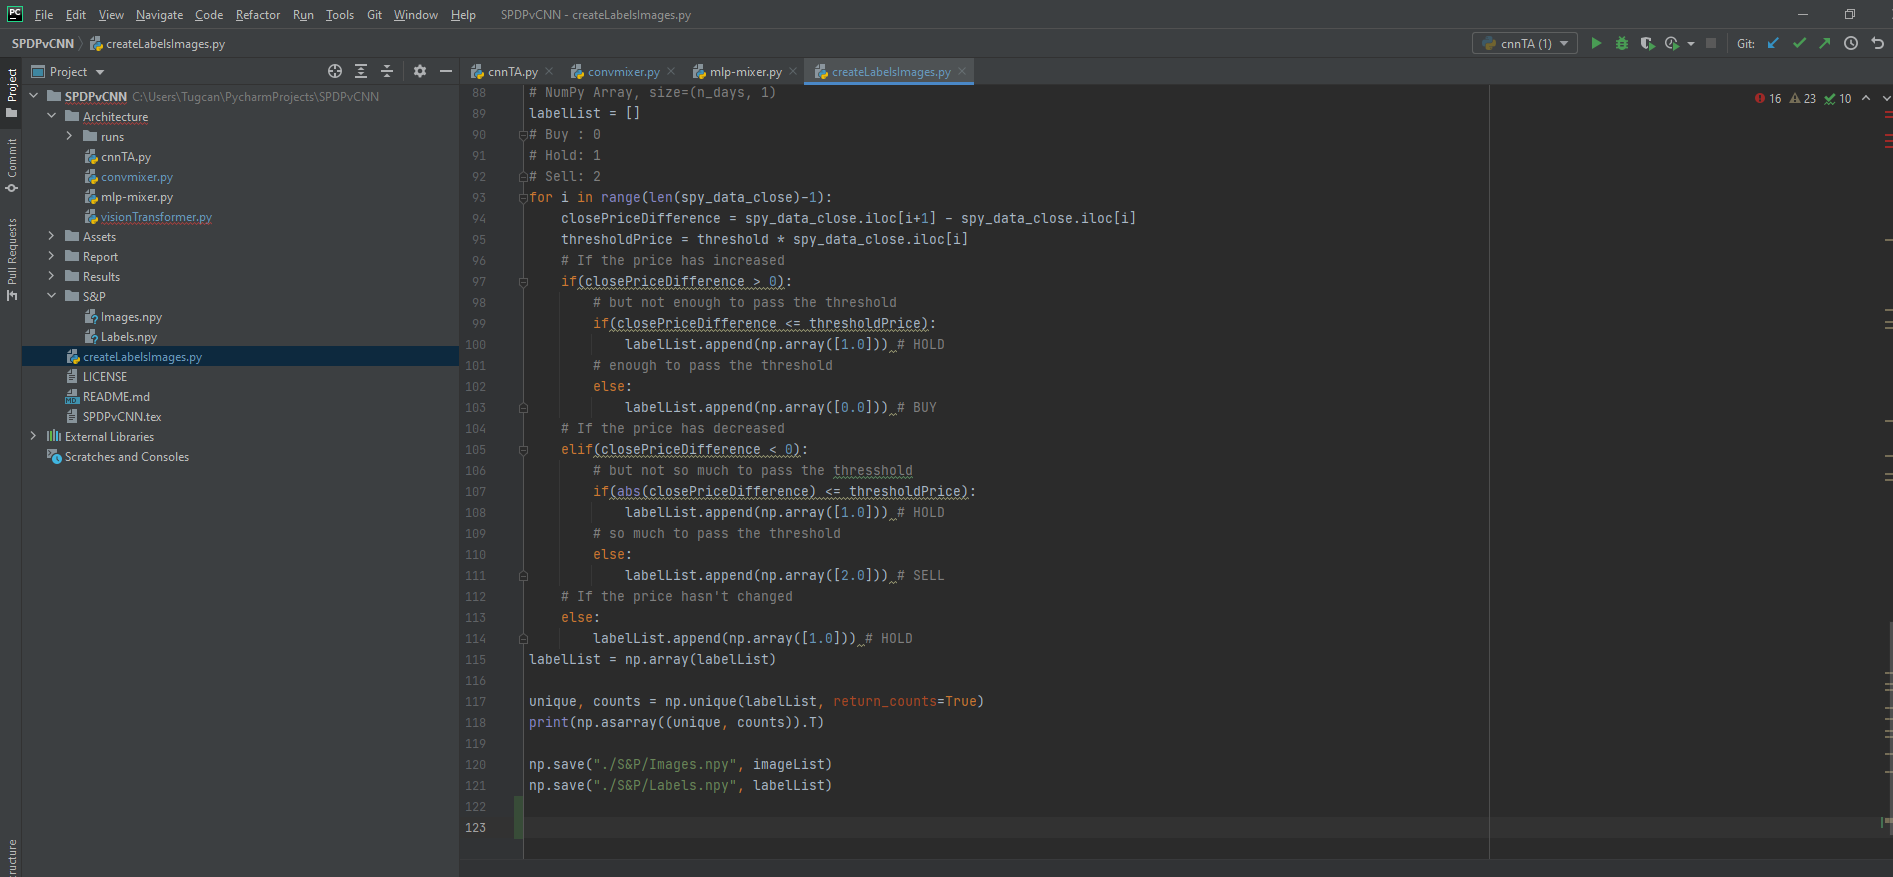
\includegraphics[scale=0.155]{assets/appendix/image_creation_alg.png}
    \caption{Algorithm of Labeling}
\end{center}
\end{figure}
\noindent
\begin{figure}[H]
\begin{center}
    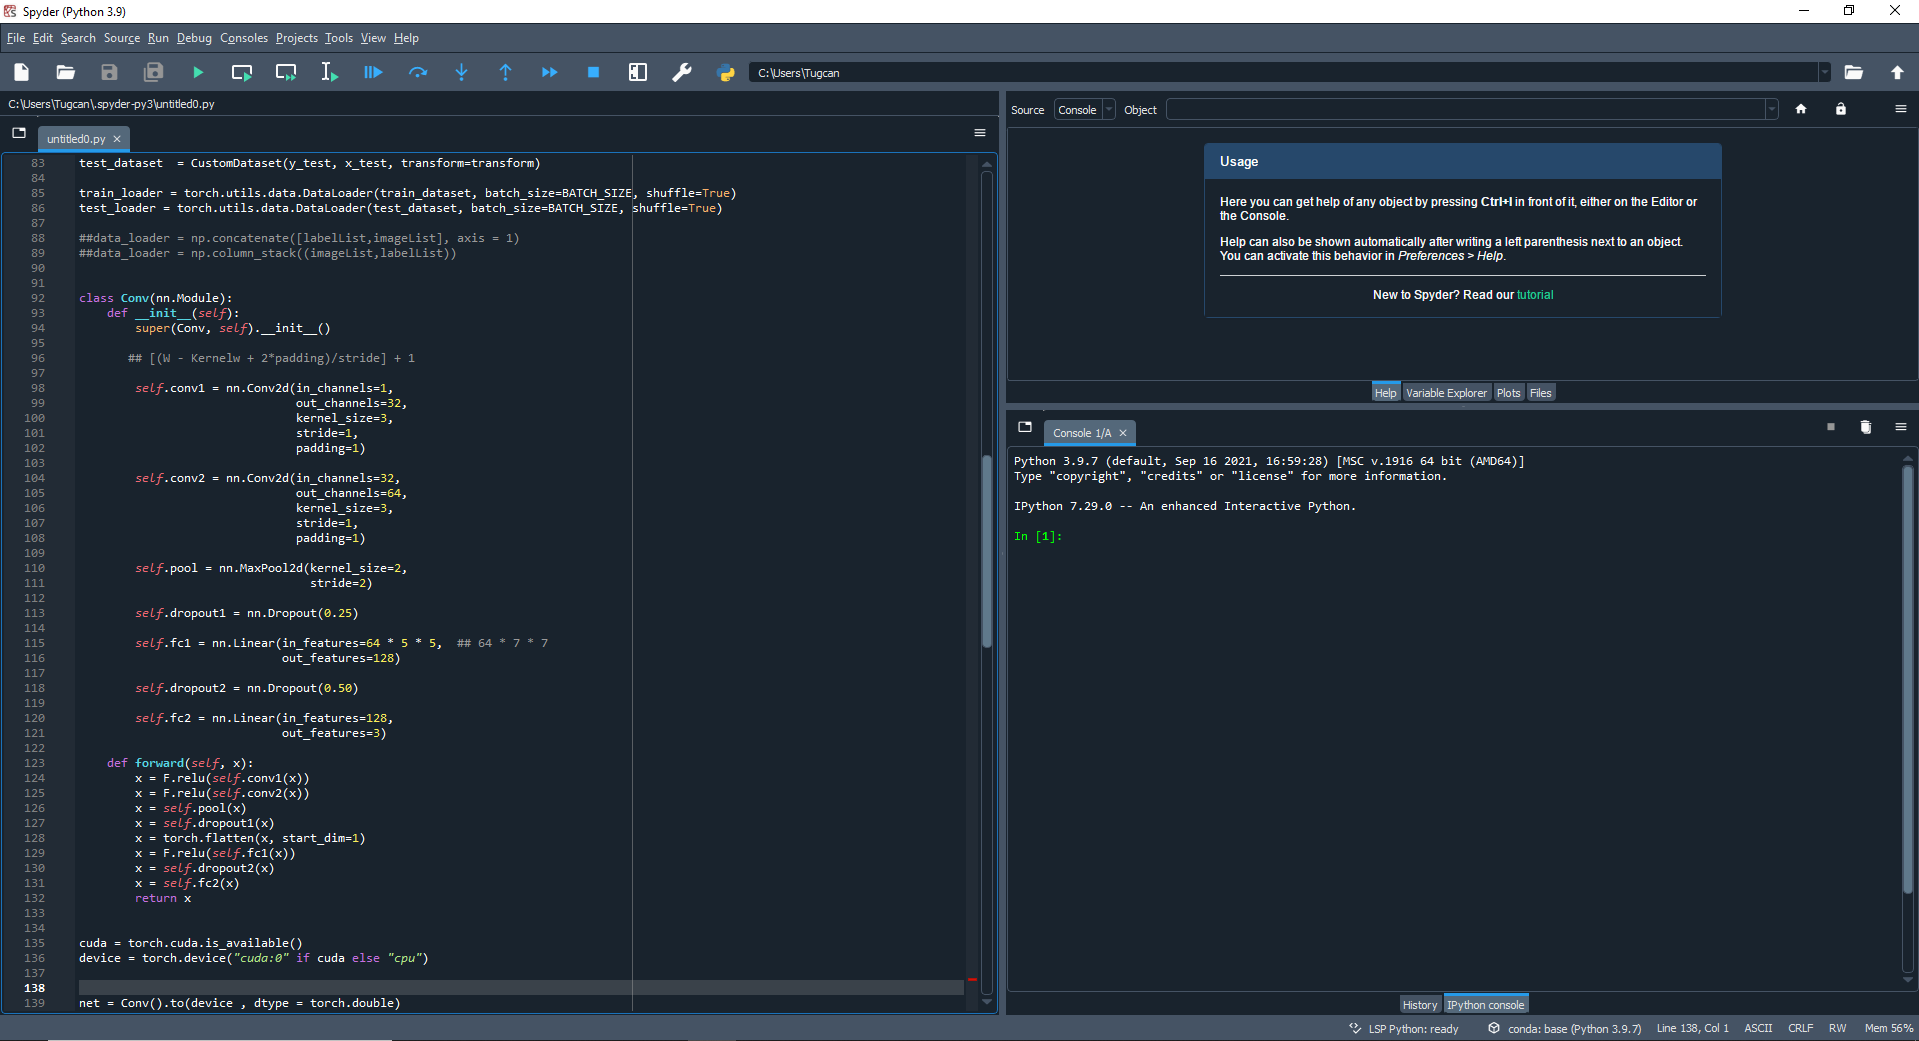
\includegraphics[scale=0.18]{assets/appendix/cnn_implemantation.png}
    \caption{Algorithm of Convolutional Neural Network}
\end{center}
\end{figure}
\noindent
\begin{figure}[H]
\begin{center}
    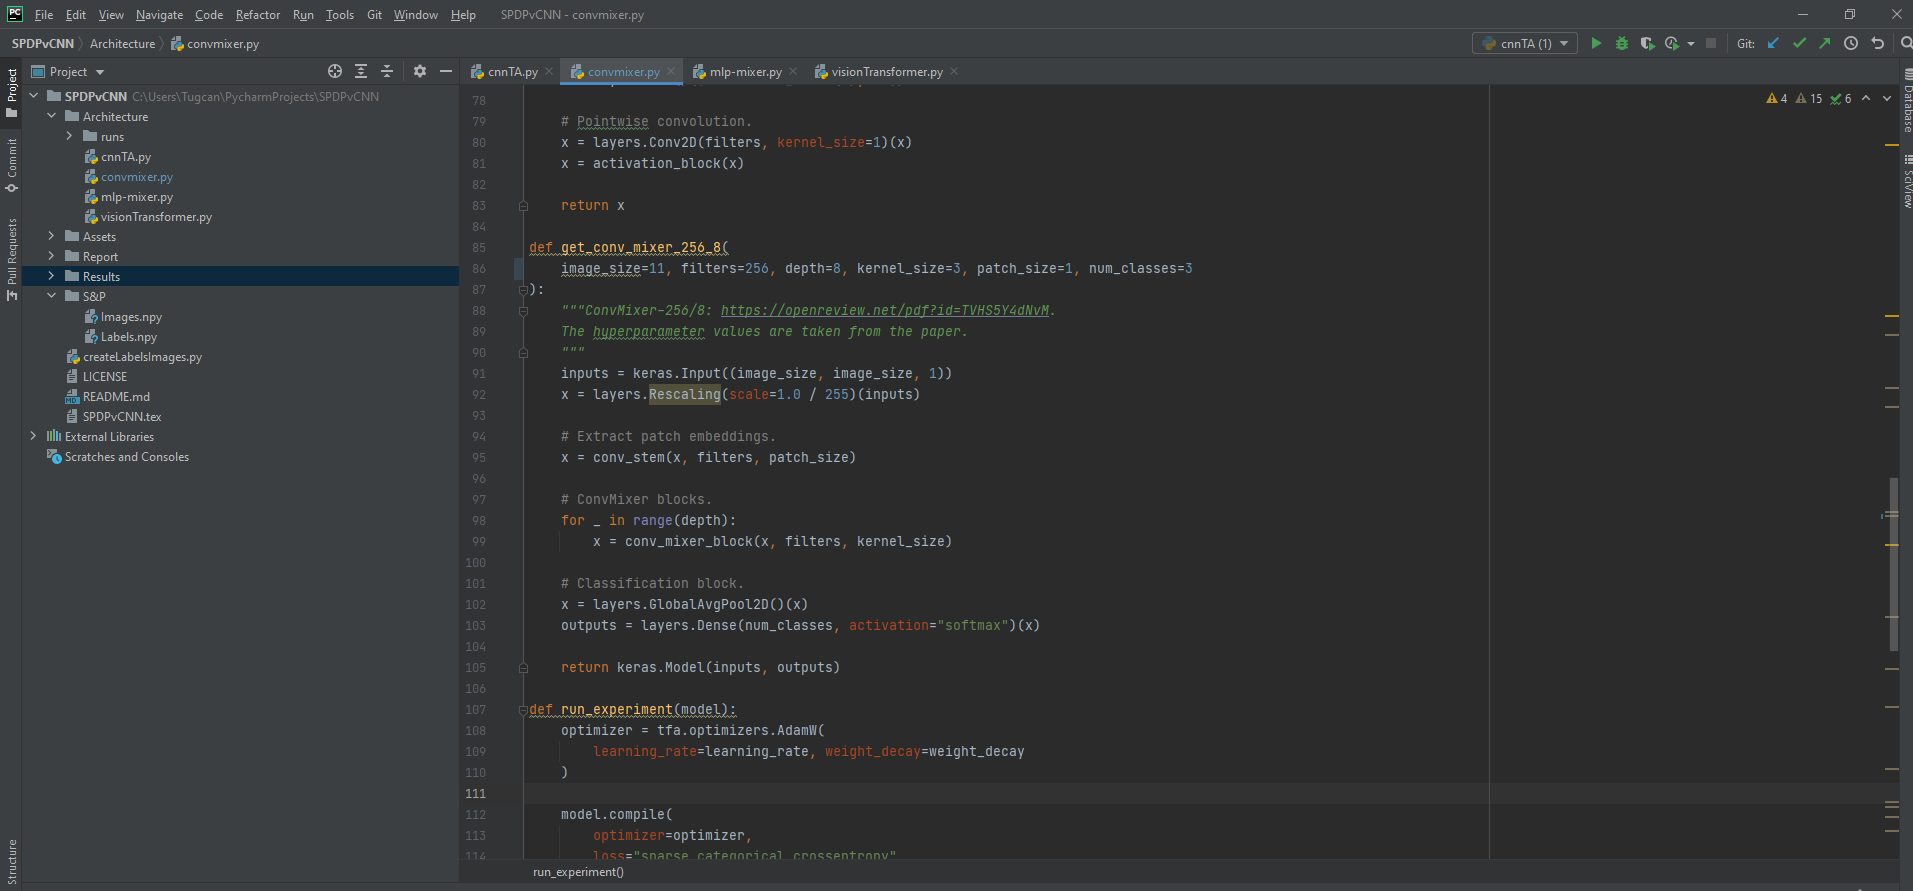
\includegraphics[scale=0.18]{assets/appendix/convmixer_implemantation.png}
    \caption{Algorithm of ConvMixer}
\end{center}
\end{figure}
\noindent
\begin{figure}[H]
\begin{center}
    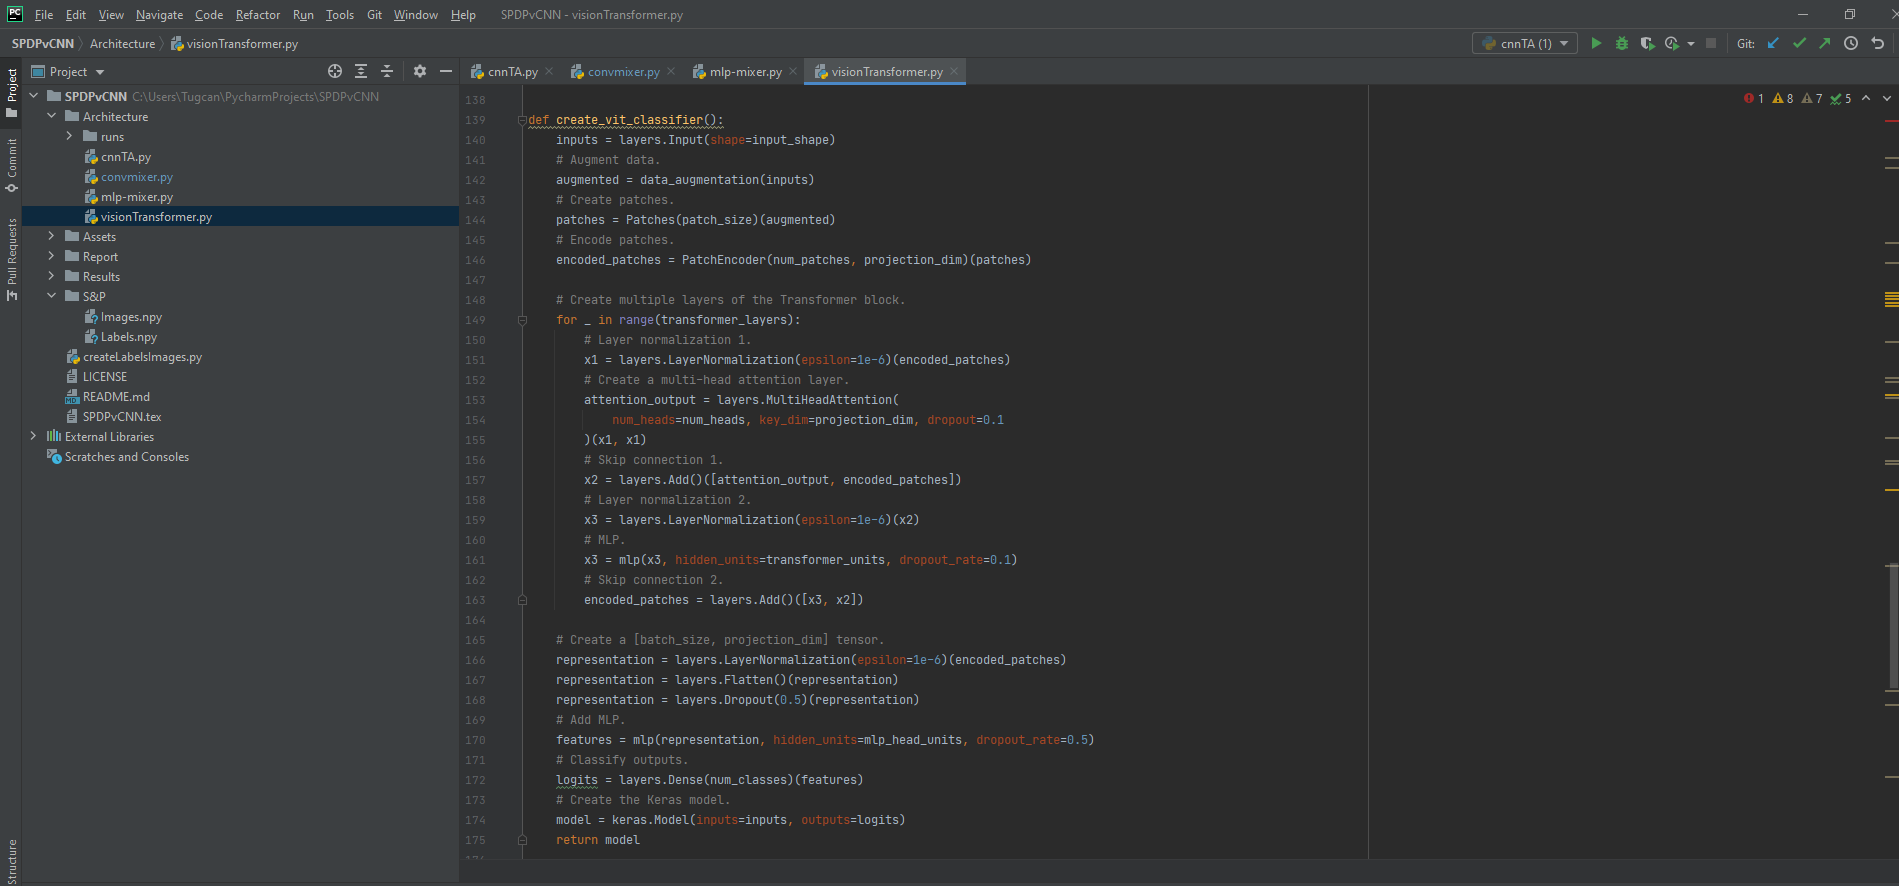
\includegraphics[scale=0.15]{assets/appendix/vit_implemantation.png}
    \caption{Algorithm of Vision Transformer}
\end{center}
\end{figure}
\noindent
\end{document}
